\section{Treap}
    這應該是第一個單元標題是英文的了。不過他有中文名,樹堆

    \subsection{前言}

    Treap 是一個隨機平衡的二元搜尋樹,
    這裡所說的 Treap 是以 merge/split 的方式實作的,
    這樣實作的 Treap 有很多好處,我們先說明他的基本規則,
    以及 merge/split 函式(function)在做什麼,
    接著說明如何實作。

    樹堆的名稱來由是 樹(Tree) 和 堆積(Heap) 結合而成,
    每個節點會至少存放兩個數值 val,pri ,
     val (也有人叫他 key)就是內容,而 pri 則是用以平衡。
    
    \subsection{規則與前置作業}

    所有節點的 pri 值必須比他的左右子樹小(大也可以),
    而且樹上的 val 滿足 ``二元搜尋樹" 的性質,
    為了避免有人忘記或不知道什麼是 ``二元搜尋樹" 的性質,
    以下用一個我出過的題目說明。

    \example 第一屆卓越盃 C.Safe Sorter

    \begin{figure}[!ht]
        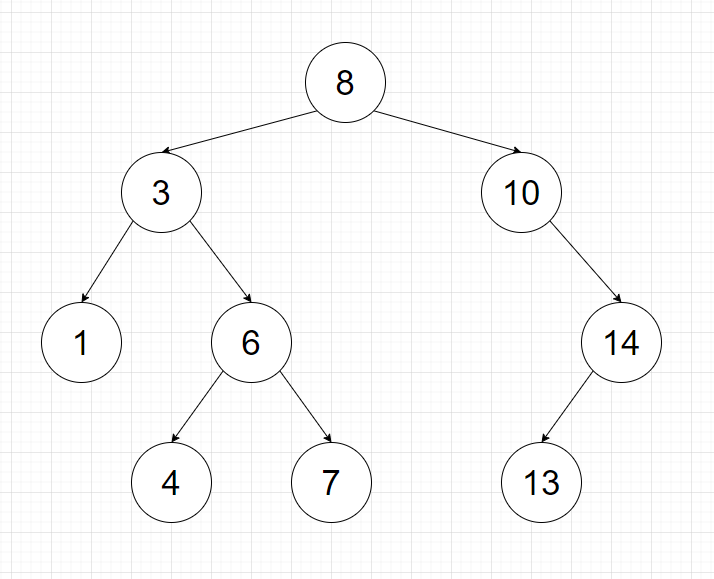
\includegraphics[width=\textwidth]{../Images/SaveSorter.png}
    \end{figure}

    \begin{itemize}
        \item 如果該節點還沒有任何保險箱,此保險箱就會佔據該節點
        \item 否則若這個要放入的保險箱裡面的金塊比在該節點的保險箱還要多,他會被往右邊送
        \item 否則就往左邊送
        \item 必須送到他占用一個節點為止
    \end{itemize}

    如圖

    \begin{itemize}
        \item 第一個放進來的保險箱有 8 個金塊
        \item 第二個有 10 個,因此他被放在右邊
        \item 第三個有 14 個,因此第一步會先往右送,發現右邊的節點也有保險箱了,因而再次被往右送
        \item 第四個有 3 個,於是被放在左邊
        \item 其他依此類推
    \end{itemize}

    而所謂隨機平衡就是他的平衡方式來自所有節點被賦予的一個隨機的 pri 值。
    Treap 當中最重要的就是以下兩種操作,並且其中一種與pri有關。

    \begin{itemize}
        \item merge(a,b) : 將兩顆樹 a, b 合併。前提 : a, b 滿足所有在 a 裡面的節點所存放的值皆小於所有在 b 裡面的節點
        \item split(a,b,p) : 將一棵樹分成 a, b 並同時滿足 a 中的值皆小於等於 $(\le)$ p , 而 b 中的值皆大於 $(>)$ p
    \end{itemize}

    兩者詳細步驟是依照遞迴定義的,首先是merge。

    \textbf{merge}

    \begin{itemize}
        \item 如果 a,b 至少其中一個是空指標,回傳非空的那一個 (兩個都空救回傳空指標)
        \item 否則為了同時維持 BST 和 heap 的性質,我們先判斷哪一個的 pri(priority) 值更大,我的實作是將 pri 值小的放上面 (較接近樹根的位置)
        \item 如果 a 的 pri 值較小,我們會回傳 a 作為呼叫此函數的樹的根,不過在此之前,我們要先決定 a 的右子樹 (因為 b 也還沒被合併完) ,所以要向下遞迴
        \item b 的情況剛好相反,因為 b 裡面的值都大於 a 裡面的值
    \end{itemize}

    \textbf{split}

    split 較為複雜,因為同時要滿足 Treap 的兩種性質。

    \begin{itemize}
        \item 若 T(要被分割的 Treap) 為空指標的話,代表整棵樹都被分完了,因此將 a,b 都設為空指標。
        \item 否則一樣要分成兩個條件 : T 的根結點的值小於等於 p ,和大於 p
        \item 如果 T 的根結點的值小於等於 p ,選擇將 T 的根結點與他的左子樹給 a 並繼續向下分解 T 的右子樹給 a 的右子樹與 b
        \item 否則將 T 的根結點與他的右子樹給 b 並繼續向下分解 T 的左子樹給 b 的左子樹與 a
    \end{itemize}

    \textbf{名次樹}

    首先介紹一下名次樹,名次樹是透過在節點內多存一個數值 $\to$ 子樹大小(size),以實現更多功能,例如 : k 在這棵樹裡面排第幾,刪除比 k 大的第一個數,還有排名第 k 的樹為何等。

    為了在 Treap 中實現這個功能,我們要多實作兩個函數 $\to$ pull \& SplitBySize(splitSz)。

    首先,我先將節點完整的 struct ,還有尋找某個指標底下的樹的 size 的函式寫出來,方便後續講解。順帶一題,為了維持名次樹的正確性,每次只要樹有經過更動就要 執行 pull 。

\begin{lstlisting}[caption=node of Treap]
struct node{
    // key 是排序依據
    // pri 是 heap 的依據
    int key,pri,sz;
    node *lch,*rch;
    
    node(int _key){
        key=_key;
        sz=1;
        lch=rch=nullptr;
        // RandomInt() 之後會實作
        pri=RandomInt();
    }
    
    void pull(){
        // 自己也算
        sz=1;
        // 判斷式相當於 lch!=nullptr
        // 要加上左右子樹的大小才是完整的
        if(lch) sz+=lch->sz;
        if(rch) sz+=rch->sz;
    }
};

int fs(node *a){
    // 如果 a 為空指標則 sz(回傳值) 為 0
    return a ? a->sz : 0;
}
\end{lstlisting}

    \textbf{SplitBySize}

    這個函式會與 Split 有點像,差別在於分開的依據不同, SplitBySize 會將整棵樹分為 a, b , 其中 a 存有前 s 小的所有數, b 則存剩下的。詳細步驟如下。

    \begin{itemize}
        \item 與 Split 相同,若 T 為空則表示分完,將 a,b 都設為空指標
        \item 否則如果 T 的左子樹的元素個數不到 s ,將 T 和他的左子樹都給 a ,然後繼續從 T 的右子樹當中切出 $s-( T 的左子樹大小)-1( T 自己)$ 個元素給 a 的右子樹
        \item 否則將 T 和他的右子樹都給 b ,然後從 T 的左子樹當中切出 s 個元素給 a
    \end{itemize}

    \textbf{隨機數}
    
    C++ 本身就有內建隨機函式可供取用。就直接放在下面供大家參考。

\begin{lstlisting}[caption=C++隨機數]
// 簡單作法,但可能被 hack
#include<crand>

int RandomInt(){
    return rand();
}

// 較長,但較不易被破解
#include<random>

unsigned seed=chrono::steady_clock().now().time_since_epoch().count();
mt19937 rng(seed);

int RandomInt(){
    return rng();
}
\end{lstlisting}

    最後附上程式碼。

\begin{lstlisting}[caption=Treap 核心]
node *merge(node *a,node *b){
    if(!a || !b) return a ? a : b;

    if(a->pri < b->pri){
        a->rch=merge(a->rch,b);
        a->pull();
        return a;
    }else{
        b->lch=merge(a,b->lch);
        b->pull();
        return b;
    }
}

void split(node *T,node *&a,node *&b,int p){
    if(!T){
        a=b=nullptr;
        return;
    }
    
    if(T->key <= p){
        a=T;
        split(T->rch,a->rch,b,p);
        a->pull();
    }else{
        b=T;
        split(T->lch,a,b->lch,p);
        a->pull();
    }
}

void splitSz(node *T,node *&a,node *&b,int s){
    if(!T){
        a=b=nullptr;
        return;
    }

    if(fs(T->lch)<s){
        a=T;
        splitSz(T->rch,a->rch,b,s-fs(T->lch)-1);
        a->pull();
    }else{
        b=T;
        splitSz(T->lch,a,b->lch,s);
        b->pull();
    }
}
\end{lstlisting}

    \subsection{基本功能}

    有了這些函式之後,後面的大多數操作都會變很簡單,
    舉凡插入(insert),刪除(erase),尋找(find) 等等。
    因為他們都可以用 merge and split 湊出來。
    而且很多功能甚至不只有一種實作方法。讓我們看下去。

    \textbf{Insert}

    insert 可以被簡單地分成幾個步驟。假設我要插入的數字為 v 。

    \begin{itemize}
        \item 將整棵樹(我都存在 rt 指標中) 切成小於等於 v 和大於 v 的兩棵樹 rt, b
        \item 另外用 v new 一個節點 a(v) 出來 (不會動態記憶體分配的可以先去複習一下)。
        \item 合併 rt 和 a ,並將合併後的樹給 rt 
        \item 合併 rt 和 b ,並將合併後的樹給 rt
    \end{itemize}
    
    \textbf{Erase}

    erase 一樣可以被簡單地分成幾個步驟。假設我要刪除的數字為 v 。

    1. 刪除所有等於 v 的數(整數才可以) 

    \begin{itemize}
        \item 將整棵樹(我都存在 rt 指標中) 切成小於等於 v 和大於 v 的兩棵樹 rt, b
        \item 再將 rt 指向的樹切成小於等於 v-1 和大於 v-1 的兩棵樹 rt, a
        \item 刪除 a 整棵樹 
        \item 合併 rt 和 b ,並將合併後的樹給 rt
    \end{itemize}

    2. 刪除一個等於 v 的數(整數才可以) 

    \begin{itemize}
        \item 將整棵樹(我都存在 rt 指標中) 切成小於等於 v-1 和大於 v-1 的兩棵樹 rt, b
        \item 再將 b 指向的樹切成左邊一個元素,剩下都放右邊的 b, a 
        \item 刪除 b 
        \item 合併 rt 和 b ,並將合併後的樹給 rt
    \end{itemize}

    如果是浮點數可能要換方法,不過基本上不會用到。

    \textbf{Count}

    假設我要數的數字為 v ,就是問v有幾個。

    \begin{itemize}
        \item 將整棵樹(我都存在 rt 指標中) 切成小於等於 v 和大於 v 的兩棵樹 rt, b
        \item 再將 rt 指向的樹切成小於等於 v-1 和大於 v-1 的兩棵樹 rt, a
        \item 用一個變數將 a 的 size 存起來
        \item 合併 rt 和 a ,並將合併後的樹給 rt 
        \item 合併 rt 和 b ,並將合併後的樹給 rt
    \end{itemize}

    \textbf{Kth Small Element}

    假設我要找第 p 小的數字。

    \begin{itemize}
        \item 將整棵樹(我都存在 rt 指標中) 切成左邊 p 個元素,剩下都放右邊的 rt, b 
        \item 再將 rt 指向的樹切成左邊 p-1 個元素,剩下都放右邊的 rt, a 
        \item 用一個變數將 a 的值存起來
        \item 合併 rt 和 a ,並將合併後的樹給 rt 
        \item 合併 rt 和 b ,並將合併後的樹給 rt
    \end{itemize}

    最後附上程式碼。

\begin{lstlisting}[caption=Treap 基本功能]
void insert(int v){
    node *a=new node(v),*b;
    split(rt,rt,b,v);
    rt=merge(rt,a);
    rt=merge(rt,b);
}

// 這個函式是先刪除左右子樹,再刪除自己,並透過遞迴來刪掉整棵樹。
void delete_tree(node *n){
    if(n->lch) delete_tree(n->lch);
    if(n->rch) delete_tree(n->rch);
    delete(n);
}

// erase all element between (v-1~v] -> 對應 1
void erase(int v){
    node *a,*b;
    split(rt,rt,b,v);
    split(rt,rt,a,v-1);// or v-eps
    // it's better to use delete_tree function
    delete(a);
    rt=merge(rt,b);
}

// erase one element between (v-1~v] -> 對應 2
void erase(int v){
    node *a,*b;
    split(rt,rt,b,v-1);
    splitSz(b,b,a,1);
    delete(b);
    rt=merge(rt,b);
}

int count(int v){
    node *a,*b;
    split(rt,rt,b,v);
    split(rt,rt,a,v-1);// or v-eps
    int ret=fs(a);
    rt=merge(rt,a);
    rt=merge(rt,b);
    return ret;
}

int kth(int v){
    node *a,*b;
    splitSz(rt,rt,b,p);
    splitSz(rt,rt,a,p-1);
    int ret=a->key;
    rt=merge(rt,a);
    rt=merge(rt,b);
    return ret;
}
\end{lstlisting}

    說到這邊,你以為只是平衡樹嗎?不不不,祂可厲害了。

    \subsection{進階功能}

    如果我們將整棵樹的中序遍歷當成序列的順序的話(如下圖),我們可以實現需多更強大的功能。
    可以說,線段樹能做到的事 Treap 都可以做到,
    但 Treap 甚至可以做到許多線段樹做不到的事。

    \begin{figure}[!htbp]
        \centering
        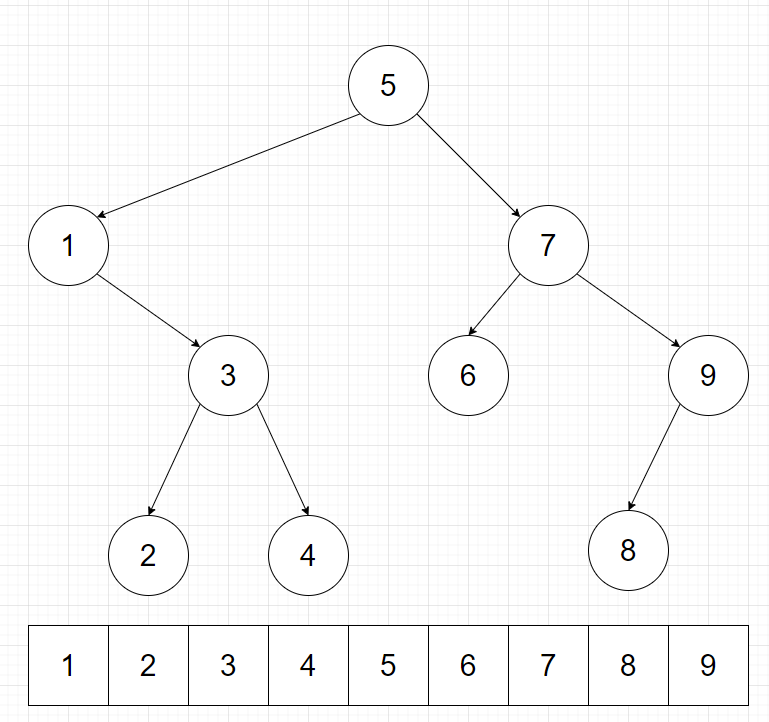
\includegraphics[width=0.6\textwidth]{../Images/Treap1.png}
        \caption{Treap 表示數列示意圖}
    \end{figure}

    而且,此時我們可以把 key 拔掉。然後只使用 splitSz 和 merge 。

    \textbf{Insert}

    假設我希望插入的數字位於第 p 個,且值為 v 。

    \begin{itemize}
        \item 將整棵樹(我都存在 rt 指標中) 切 p-1 個給 rt ,其他剩下的分給 b 
        \item 另外用 v new 一個節點 a(v) 出來
        \item 合併 rt 和 a ,並將合併後的樹給 rt 
        \item 合並 rt 和 b ,並將合併後的樹給 rt
    \end{itemize}

    \textbf{Erase}

    假設我要刪除第 p 個數。

    \begin{itemize}
        \item 將整棵樹(我都存在 rt 指標中) 切 p-1 個給 rt ,其他給 b
        \item 再將 b 指向的樹切一個給 b 剩下給 a
        \item 刪除 a 
        \item 合併 rt 和 b ,並將合併後的樹給 rt
    \end{itemize}

    \textbf{區間操作}

    在介紹區間操作之前,我們還需要在節點上加入更多的資訊和函式,所以 node 裡面會有更多程式碼。
    (以下程式碼加上了很多功能,實際上不需要那麼多)

\begin{lstlisting}[caption={Treap 表示數列使用的 node}]
const int INF=0x3f3f3f3f

struct Treap{
    struct node{
        // 此節點的值
        int val;
        // 維持 Treap 的性質
        int pri,sz;
        // 用在區間查詢
        int sum,mx,mn;
        // 可以支援區間反轉
        bool rev_tag;
        // 可以支援區間加值
        int add_tag;
        // 左右子樹
        node *lch,*rch;
        
        node(int _val){
            val=sum=mx=mn=_val;
            lch=rch=nullptr;
            sz=1;
            pri=rng();
        }
        
        void pull(){
            sz=1;
            sum=mx=mn=val;
            
            if(lch){
                sz+=lch->sz;
                sum+=lch->sum;
                mx=max(mx,lch->mx);
                mn=min(mn,lch->mn);
            }
            
            if(rch){
                sz+=rch->sz;
                sum+=rch->sum;
                mx=max(mx,rch->mx);
                mn=min(mn,rch->mn);
            }
        }
        
        // 讓他底下的區間都反轉
        void rev(){
            rev_tag=!rev_tag;
        }
        
        // 再更改節點前用
        void push(){
            if(rev_tag){
                swap(lch,rch);
                if(lch)
                    lch->tag=true;
                if(rch)
                    rch->tag=true;
            }
            
            if(lch)
                lch->add_tag+=add_tag;
            if(rch)
                rch->add_tag+=add_tag;
            add_tag=0;
        }
    };
};
\end{lstlisting}

    同時,我們在原來的 merge/split 操作程式碼中,都要加上 push ,具體位置如下。

\begin{lstlisting}[caption=push 放的位置]
struct Treap{
    node *merge(node *a,node *b){
        if(!a || !b) return a ? a : b;

        if(a->pri < b->pri){
            a->push();
            a->rch=merge(a->rch,b);
            return a;
        }else{
            b->push();
            b->lch=merge(a,b->lch);
            return b;
        }
    }
    
    void splitSz(node *T,node *&a,node *&b,int s){
        if(!T){
            a=b=nullptr;
            return;
        }

        T->push();
        
        if(fs(T->lch)<s){
            a=T;
            splitSz(T->rch,a->rch,b,s-fs(T->lch)-1);
            a->pull();
        }else{
            b=T;
            splitSz(T->lch,a,b->lch,s);
            b->pull();
        }
    }
};
\end{lstlisting}

    接下來的操作都是把區間切下來,做完我要做的事,再接回去就可以了。

    \textbf{區間查詢(極值、總和)}

    假設現在要查詢 $[l,r]$ 的區間。

    \begin{itemize}
        \item 從 rt 切下 r 個節點給 rt ,其它給 b 
        \item 接著從 rt 切下 l-1 個節點給 rt ,其餘給 a
        \item 此時 a 就存有區間 $[ l, r ]$ ,而他的 sum, mx, mn 就會是這個區間的總和、最大值,以及最小值
        \item 最後先按照順序把它合併,再回傳答案即可
    \end{itemize}

    \textbf{單點修改}

    先將所要修改的位置切下來,修改完後merge回去,在修改完後記得要 push 。

    \textbf{區間操作}

    假設現在要對 $[l,r]$的區間進行操作。

    \begin{itemize}
        \item 從 rt 切下 r 個節點給 rt ,其它給 b 
        \item 接著從 rt 切下 l-1 個節點給 rt ,其餘給 a
        \item 此時 a 就存有區間 $[l, r]$ ,直接對他操作就可以了
        \item 最後先按照順序把它合併
    \end{itemize}

    當然,與線段樹相同,區間操作通常需要懶人標記。

    最後附上程式碼。

\begin{lstlisting}[caption=Treap進階操作]
int query(int l,int r){
    node *a,*b;
    splitSz(rt,rt,b,r);
    splitSz(rt,rt,a,l-1);
    // 下一行放 sum, mx, mn 看需求
    int ret=a->sum;
    rt=merge(rt,a);
    rt=merge(rt,b);
    return ret;
}

// 單點查詢就用查詢長度為 1 的區間重復利用函式就可以了
// 不過會比較慢
int get(int p){
    return query(p,p); 
}

void modify(int p,int v){
    node *a,*b;
    splitSz(rt,rt,a,p-1);
    splitSz(a,a,b,1);
    a->val=v;
    rt=merge(rt,a);
    rt=merge(rt,b);
}

// 區間反轉
void reverse(int l,int r){
    node *a,*b;
    splitSz(rt,rt,b,r);
    splitSz(rt,rt,a,l-1);
    if(a) a->rev();
    rt=merge(rt,a);
    rt=merge(rt,b);
}

// 區間加值
void add(int l,int r,int v){
    node *a,*b;
    splitSz(rt,rt,b,r);
    splitSz(rt,rt,a,l-1);
    a->val+=v;
    a->push();
    rt=merge(rt,a);
    rt=merge(rt,b);
}
\end{lstlisting}

    \subsection{解構式}
    對於多筆測資,可能會需要釋放記憶體。
    由於 Treap 二元樹的特性,可以透過遞迴刪除整棵樹。

\begin{lstlisting}[caption=Treap 解構式]
void DeleteTree(node *n){
    if(n->lch) DeleteTree(n->lch);
    if(n->rch) DeleteTree(n->rch);
    delete(n);
}

~Treap(){
    if(rt) DeleteTree(rt);
}
\end{lstlisting}

    \subsection{一些神奇的東西}
    因為幾乎不會用到,只是好玩寫的,所以不解釋。

\begin{lstlisting}[caption=其他功能]
int size(){
    return fs(rt);
}

bool empty(){
    return size()==0;
}

void push_back(num v){
    insert(size()+1,v);
}

void push_front(num v){
    insert(1,v);
}

void pop_back(){
    erase(size()+1);
}

void pop_front(){
    erase(1);
}

void resize(int sz){
    while(size()<sz){
        push_back(0);
    }
    while(size()>sz){
        pop_back();
    }
}

void resize(int sz,num v){
    while(size()<sz){
        push_back(v);
    }
    while(size()>sz){
        pop_back();
    }
}

Treap(){}
Treap(int sz){
    resize(sz);
}

Treap(int sz,int v){
    resize(sz,v);
}
\end{lstlisting}

    \subsection{持久化}
    正在研究$\cdots$

    \subsection{小結}

    Treap 還有更多操作可以使用,我並未,也不可能一一列舉。你們只要記得
    merge和split可以創造出無限可能。

    不過小心,Treap會使用大量記憶體與時間。雖然同樣是$O(\log{(n)})$。
    同級距下Treap會比較慢,當然,有一些用值域線段樹的問題,用Treap會跑的比較快,
    畢竟這次複雜度不相同了$O(\log C) > O(\log n), C \le 10^{12}, n \le 10^5$。

    \subsection{範例與練習}

    \problem 第一屆卓越盃 F.Safe Sequence(Hard)

    \textbf{題目敘述}

    你是一家銀行負責保管保險箱的保險箱管理處處長,由於最近銀行生意並不是非常好,因此銀行行長決定跟員工玩一個遊戲。以下為遊戲會用到的操作。

    \begin{enumerate}
        \item 新增一個保險箱到保險箱序列第 $x$ 個後面,且該保險箱此時已經有 $y$ 個金條 
        \item 反轉 $[l,r]$ 的保險箱 ~註1~ 
        \item 詢問區間 $[l,r]$ 的金條總數
        \item 從目前保險箱序列中的第 $x$ 個位置拿出 $y$ 個金條 
        \item 在目前保險箱序列中的第 $x$ 個位置放入 $y$ 個金條 
    \end{enumerate}

    \textbf{輸入說明}

    第一行輸入 $1$ 個數字 $t$ ,代表有 $t$ 比測試資料
    
    每筆測資第一行輸入 $2$ 個數字 $n,q$ ,表示一開始的保險箱有幾個
    
    第二行輸入 $n$ 個數字 $a_1,a_2...a_n$ , $a_i$ 代表第 $i$ 個保險箱原來有幾塊金條
    
    接下來有 $q$ 行,分別對應一個操作(以下說明)

    對應題目敘述的第 $k$ 項操作

    \begin{enumerate}
        \item 輸入 $1$ $x$ $y$
        \item 輸入 $2$ $l$ $r$
        \item 輸入 $3$ $l$ $r$
        \item 輸入 $4$ $x$ $y$
        \item 輸入 $5$ $x$ $y$
    \end{enumerate}

    $t \le 100$,$n,q,a_i,x,y \leq 10^4$

    \textbf{輸出說明}

    僅有操作 $3$ 需要輸出區間 $[l,r]$ 的金條總數

    \textbf{範例測試}

    \begin{tabular}{|m{7cm}|m{7cm}|}
        \hline
        範例輸入 1 & 範例輸出 1 \\
        \hline
        \verb|1| & \verb|10| \\
        \verb|4 2| & \\
        \verb|1 2 3 4| & \\
        \verb|2 1 4| & \\
        \verb|3 1 3| & \\
        \hline
    \end{tabular}

    註1 : 由於銀行裝備有"量子軌道位移系統",
    因此無須擔心保險箱管理處員工因搬運過多保險箱而導致橫紋肌溶解,
    或是出現保險箱太重而搬不動的問題。

    \problem CF 702F T-Shirts

    \textbf{題目敘述}

    大批量的 T 恤在商店在春季之前上架。總共有 $n$ 種 T 恤上架販售。第 $i$ 種 T 恤有兩個整數參數 — $c_i$ 和 $q_i$,其中 $c_i$ 表示第 $i$ 種 T 恤的價格,$q_i$ 表示第 $i$ 種 T 恤的品質。假設商店中有無限數量的每種 T 恤可供販售,但是通常價格和品質並無關聯。

    根據預測,在接下來的一個月內將有 $k$ 名顧客光臨該商店,第 $j$ 個顧客打算花費不超過 $b_j$ 來購買 T 恤。

    所有顧客都使用相同的策略。首先,顧客希望購買最多可能的最高品質的 T 恤,然後從剩餘的 T 恤中購買最多可能的最高品質的 T 恤,以此類推。同時,在多個品質相同的 T 恤中,顧客會選擇價格更低的那件。顧客不喜歡相同的 T 恤,因此每位顧客不會購買多於一件同款的 T 恤。

    請根據所描述的策略,確定每位顧客將購買的 T 恤數量。所有顧客之間是獨立的,一位顧客的購買不會影響其他顧客的購買。

    \textbf{輸入說明}

    第一行包含一個正整數 $n$ ($1 \leq n \leq 2 \times 10^5$) — T 恤類型的數量。

    接下來的 $n$ 行,每行包含兩個整數 $c_i$ 和 $q_i$ ($1 \leq c_i, q_i \leq 10^9$) — 第 $i$ 種 T 恤的價格和品質。

    接下來一行包含一個正整數 $k$ ($1 \leq k \leq 2 \times 10^5$) — 顧客的數量。

    接下來一行包含 $k$ 個正整數 $b_1, b_2, \cdots, b_k$ ($1 \leq b_j \leq 10^9$),其中第 $j$ 個數字表示第 $j$ 位顧客打算花費的總金額。

    \textbf{輸出說明}

    輸出的第一行應包含一個長度為 $k$ 的整數序列,其中第 $i$ 個數字應該等於第 $i$ 位顧客將購買的 T 恤數量。

    \textbf{範例測試}

    \begin{tabular}{|m{7cm}|m{7cm}|}
        \hline
        範例輸入 1 & 範例輸出 1 \\
        \hline
        \verb|3| & \verb|2 3| \\
        \verb|7 5| & \\
        \verb|3 5| & \\
        \verb|4 3| & \\
        \verb|2| & \\
        \verb|13 14|& \\
        \hline
    \end{tabular}

    \problem TIOJ 1382 約瑟問題

    \textbf{題目敘述}

    還記得約瑟夫問題嗎!? 沒錯就是那位約瑟夫人。這次問題是約瑟問題,不是約瑟夫問題唷!!

    有個古老的經典問題是這樣的:
    n 個人圍成圓圈,從頭開始每 k 個一數殺掉,最後問 Joseph 今天晚餐吃什麼。

    很難對吧。今天問題簡單多了,而且是普遍級的,不殺人的

    有 n 個人依照編號順去坐著圍成圓圈,每個人的椅子都被裝上``強制脫出裝置" 
    ,接著有張神秘的紙條上面寫著 n 個數,代表每一次要數幾個人之後彈出(開始時從第一位開始數)

    \textbf{輸入說明}

    包含多組測試資料,請以EOF做為結束(測試資料不超過10組)

    每筆測試資料的第一行為一個數字 n 代表有多少人

    第二行有n個數字$a_1,a_2, \cdots , a_n$,$a_i$ 代表第$i$次數到第$a_i$個人被彈出
    
    $1 \le n,a_i \le 10^5$

    \textbf{輸出說明}

    輸出彈出的順序,編號是$1$~$n$。

    \textbf{範例測試}

    \begin{tabular}{|m{7cm}|m{7cm}|}
        \hline
        範例輸入 1 & 範例輸出 1 \\
        \hline
        \verb|5| & \verb|2 5 3 4 1| \\
        \verb|2 3 2 3 1| & \\
        \hline
    \end{tabular}